
\section{Results and Analysis}
A single \gls{cnn} was used as a means to control the experiments. For this, Sphereface~\cite{liu2017sphereface} trained on CASIA-Web~\cite{yi2014learning}, and evaluated on \gls{lfw}~\cite{LFWTech} (\%99.22 accuracy), encoded all of the faces.\footnote{\href{$https://github.com/clcarwin/sphereface\_pytorch$}{https://github.com/clcarwin/sphereface\_pytorch}} As reported in~\cite{wang2019racial}, \gls{lfw} has about a 13\%, 14\%, 3\%, and 70\% ratio in Asian, Black, Indian, and White, respectively. Furthermore, CASIA-Web is even more unbalanced (again, as reported in~\cite{wang2019racial}), with about  3\%, 11\%, 2\%, and 85\% for the same subgroups.
%\vspace{-4mm}
\glsunset{det}
% \subsection{\gls{det} analysis}
\noindent\paragraph{\gls{det} analysis.}
\gls{det} curves (5-fold, averaged) show per-subgroup trade-offs (Fig.~\ref{fig:detcurves}). Note that \gls{m} performs better than \gls{f}, precisely as one would expect from the tails of score-distributions for \emph{genuine} pairs (Fig.~\ref{fig:detection-model}). \Gls{af} and \gls{if} perform the worst.
\glsunset{m}
\glsunset{f}

% Specifically, we analyze three \glspl{cnn} variants: we encode faces using VGG-16~\cite{simonyan2014very},  50-layer residual network (\ie ResNet-50)~\cite{he2016deep}, and \gls{senet} (\ie SENet-50)~\cite{hu2018squeeze}, with results of only the latter (\ie the best performing \gls{senet}) model used throughout the main paper. Results for the other two, alongside \gls{senet} for comparison, are in the Supplemental Material.
%\vspace{-4mm}

\glsunset{am}\glsunset{af}\glsunset{bm}\glsunset{bf}\glsunset{im}\glsunset{if}\glsunset{wm}\glsunset{wf}
\begin{figure*}[h!]
    \centering
    \begin{subfigure}[t]{.3\linewidth}
    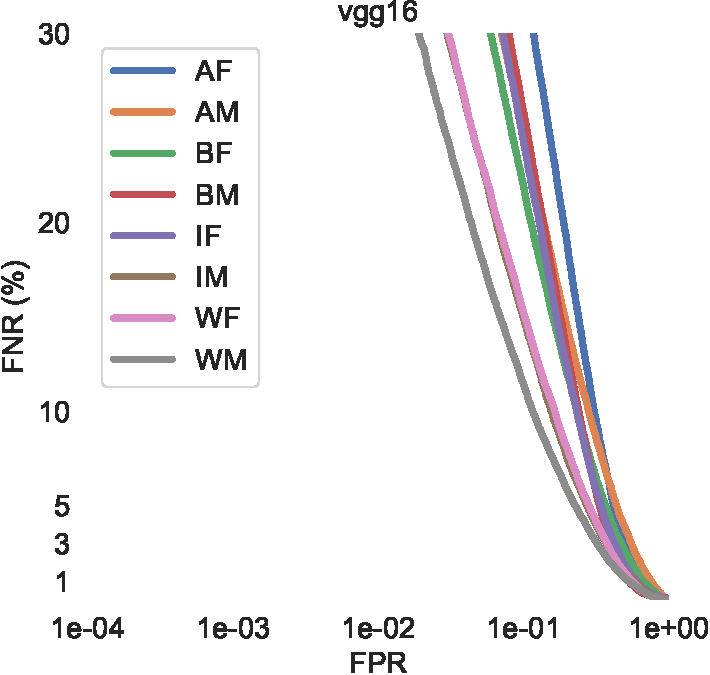
\includegraphics[width=.71\linewidth]{figures/curve_vgg16_subgroups-crop.pdf}
    \caption{VGG16~\cite{simonyan2014very}}
 \end{subfigure}
    \begin{subfigure}[t]{.27\linewidth}
    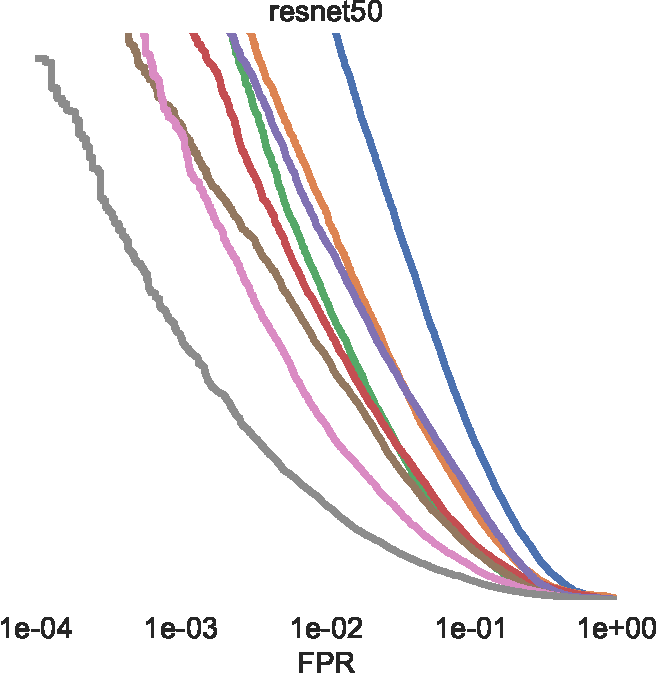
\includegraphics[width=.75\linewidth]{figures/curve_resnet50_subgroups-crop.pdf}
    \caption{ResNet50~\cite{he2016deep}}
   \end{subfigure}
    \begin{subfigure}[t]{.27\linewidth}
    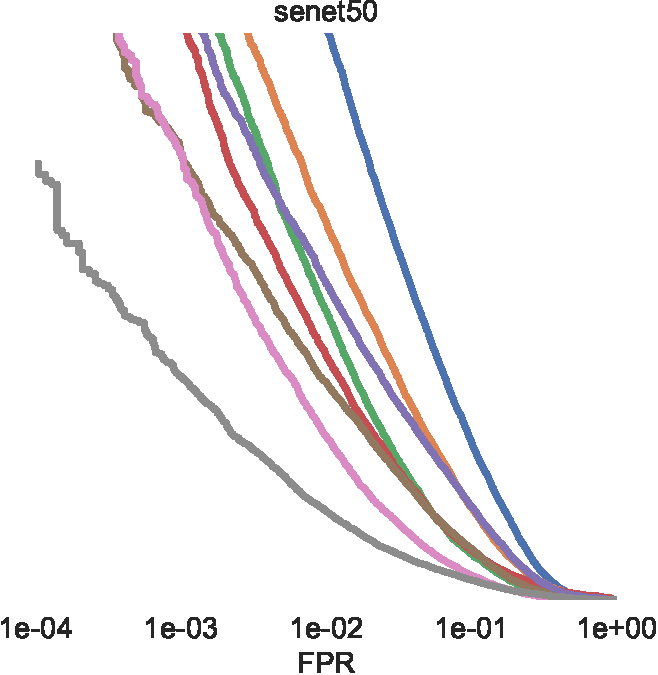
\includegraphics[width=.75\linewidth]{figures/curve_senet50_subgroups-crop.pdf}
    \caption{SENet~\cite{hu2018squeeze}}
    \end{subfigure}
    \caption{\small{\textbf{\gls{det} curves for different CNNs}. \gls{fnr} (\%) (vertical) vs \gls{fpr}  (horizontal, log-scale) for VGG2~\cite{Cao18} models with different backbones (VGG16, Resnet50, SEnet50). Lower is better. For each plot, \gls{wm} is the top-performer, while \gls{af} is the worst. The ordering of the curves is roughly the same for each backbone.}}\label{fig:sdm-appendix-a}
%    \vspace{-5mm}
\end{figure*}
\noindent\paragraph{Score analysis.}
% \subsection{Score analysis}
Fig.~\ref{fig:detection-model} shows score distributions for faces of the same (\ie \emph{Genuine}) and different (\ie \emph{Imposter}) identity, with a subgroup per \gls{sdm} plot. Notice that score distributions for imposters tend to peak about zero for all subgroups, and with minimal deviation comparing modes of the different plots. On the other hand, the score distribution of the \emph{genuine} pairs varies across subgroups in location (\ie score value) and spread (\ie overall shape). Asian Fem
Fig.~\ref{fig:confusion} shows the confusion matrix of the subgroups. A vast majority of errors occur in the intra-subgroup. It is interesting to note that while the definition of  each group  based on ethnicity and race may not be crisply defined, the confusion matrix indicates that in practice, the \gls{cnn} finds that the groups are effectively separate. The categories are, therefore, meaningful for \gls{fr}.








% \gls{det} curves averaged across 5-folds show per-subgroup trade-offs (Fig.~\ref{fig:detcurves}). Note that \gls{m} performs better than \gls{f}, precisely as one would expect from the tails of score-distributions for \emph{genuine} pairs (Fig.~\ref{fig:detection-model}). \Gls{af} and \gls{if} perform the worst.


 
\begin{table}[b!]
%    \vspace{-4mm}
\glsunset{tar}
\glsunset{far}
\caption{\small{\textbf{\gls{tar} at intervals of \gls{far}}. \gls{far}, listed are the \gls{tar} scores for a global threshold (top) and the proposed category-based threshold (bottom). Higher is better.}}\label{tab:ethnicy-far} 
% \vspace{-2mm}
\begin{center}
\scriptsize
\begin{tabular}{l c c c c c}
     \gls{far} & 0.3 & 0.1 & 0.01 & 0.001 & 0.0001\\\midrule
    \multirow{2}{.1mm}{\textbf{\gls{af}}} &0.990 & 0.867 & 0.516 & 0.470 & 0.465\\[-4pt]
        &1.000 & 0.882 & 0.524 & 0.478 & 0.474\\[-1pt]
    \multirow{2}{3mm}{\textbf{\gls{am}}} &0.994 & 0.883 & 0.529 & 0.482 & 0.477\\[-4pt]
        &1.000 & 0.890 & 0.533 & 0.486 & 0.482\\[-1pt]
    \multirow{2}{3mm}{\textbf{\gls{bf}}} &0.991 & 0.870 & 0.524 & 0.479 & 0.473\\[-4pt]
        &1.000 & 0.879 & 0.530 & 0.484 & 0.480\\[-1pt]
    \multirow{2}{3mm}{\textbf{\gls{bm}}} &0.992 & 0.881 & 0.526 & 0.480 & 0.474\\[-4pt]
        &1.000 & 0.891 & 0.532 & 0.485 & 0.480\\[-1pt]
    \multirow{2}{3mm}{\textbf{\gls{if}}} &0.996 & 0.881 & 0.532 & 0.486 & 0.481\\[-4pt]
        &1.000 & 0.884 & 0.534 & 0.488 & 0.484\\[-1pt]
    \multirow{2}{3mm}{\textbf{\gls{im}}} &0.997 & 0.895 & 0.533 & 0.485 & 0.479\\[-4pt]
        &1.000 & 0.898 & 0.535 & 0.486 & 0.481\\[-1pt]
    \multirow{2}{3mm}{\textbf{\gls{wf}}} &0.988 & 0.878 & 0.517 & 0.469 & 0.464\\[-4pt]
        &1.000 & 0.894 & 0.526 & 0.478 & 0.474\\[-1pt]
    \multirow{2}{3mm}{\textbf{\gls{wm}}} &0.989 & 0.896 & 0.527 & 0.476 & 0.470\\[-4pt]
        &1.000 & 0.910 & 0.535 & 0.483 & 0.478\\[-1pt]
    \midrule
    \multirow{2}{3mm}{\textbf{Avg.}} &0.992 & 0.881 & 0.526 & 0.478 & 0.474\\[-4pt]
        &1.000 & 0.891 & 0.531 & 0.483 & 0.479\\[-10pt]
\end{tabular}
\end{center}
\glsreset{tar}
\glsreset{far}
%  \vspace{-3mm}

\end{table}
\glsunset{fpr}

The gender-based \gls{det} curves show performances with a fixed threshold (dashed line). Other curves relate similarity (lines omitted to declutter). For many \gls{fr} applications, systems operate at the highest \gls{fpr} allowed. The constant threshold shows that a single threshold produces different operating points (\ie \gls{fpr}) across subgroups, which is undesirable. % The difference in \gls{fpr} is approximately a factor of two.
If this is the case in an industrial system, one would expect a difference in about double the FPs reported based on subgroup alone. The potential ramifications of such a bias should be considered, which it has not as of lately-- even noticed in main-stream media ~\cite{england2019,snow2018}.

To further demonstrate the extent of the problem, we follow settings typical for systems in practice. We set the desired \gls{fpr}, and then determine the percent difference, \ie desired versus actual (Fig.~\ref{fig:percent:difference}, \emph{top}). Furthermore, we mitigate this highly skewed phenomena by applying subgroup-specific thresholds (\emph{bottom}). By this, minimal error from the desired \gls{fpr}. In addition, where there is small error, the offset is balanced across subgroups.

% \subsubsection{Other \gls{cnn} models.}~\label{app:sec:other:models}
%\vspace{-5mm}
\noindent\paragraph{Model analysis.}
Variations in optimal threshold exist across models (Fig.~\ref{fig:sdm-appendix-a}). Like in Fig.~\ref{fig:detcurves}, the \gls{det} curves for three \gls{cnn}-based models, each trained on VGG2 with softmax but with different backbones.\footnote{\href{https://github.com/rcmalli/keras-vggface}{https://github.com/rcmalli/keras-vggface}} Notice similar trends across subgroups and models, which is consistent with  Sphereface as well (Fig.~\ref{fig:detcurves}). For example, the plots generated with Sphereface and VggFace2 all have the \gls{wm} curve at the bottom (\ie best) and \gls{af} on top (\ie worst). Thus, the additional \gls{cnn}-based models demonstrate the same phenomena: proportional to the overall model performance, exact in the ordering of curves for each subgroup.

%\vspace{-5mm}
\noindent\paragraph{Verification threshold analysis.}%\subsection{Verification threshold} \label{subsec:analysis:verification}
We seek to reduce the bias between subgroups. Such that an operating point (\ie \gls{fpr}) is constant across subgroups. To accomplish that, we used a per subgroup threshold. In \gls{fv}, we consider one image as the query, and all others as the test. For this, the ethnicity of the query image is assumed. We can then examine the \gls{det} curves and pick the best threshold per subgroup for a certain \gls{fpr}.

We evaluated \gls{tar} for specific \gls{far} values. As described in Section~\ref{subsec:pf}, the verification experiments were 5-fold, with no overlap in subject ID between folds. Results reported are averaged across folds in all cases and are shown in Table~\ref{tab:ethnicy-far}. For each subgroup, the \gls{tar} of using a global threshold is reported (upper row), as well as using the optimal per subgroup threshold (lower row). 

Even for lower \gls{far}, there are notable improvements, often of the order of 1\%, which can be challenging to achieve when \gls{far} is near $\geq$90\%. More importantly, each subgroup has the desired \gls{fpr}, so that substantial differences in \gls{fpr} will remain unfounded. We experimented with ethnicity estimators on both the query and test image, which yielded similar results to those reported here.

%%%%%%%%%%%%%%%%%%%%%%%%%%%%%%%%%%%%%%%%%%%%%%%%%%%%%%%%%%%%%%%%%%%%%%%%%%%%%%%%
\begin{table}[t!]
\begin{center}
    \caption{\small{\textbf{Human assessment (quantitative).} Subgroups listed per row (\ie human) and column (\ie image). Note, most do the best intra-subgroup (\textcolor{blue}{blue}), and second-best (\textcolor{red}{red}) intra-subgroup but inter-gender. WF performs the best; WF pairs are most correctly matched.}}
    % CF shows the least variation, but with the lowest accuracy. WF shows the best accuracy, in human performance and on face pairs of that subgroup.}}
    \label{tab:humsn-eval-results} 
    % \vspace{-5mm}
     \vspace{-2mm}
\footnotesize
\scalebox{0.94}{
\begin{tabular}{c}
\begin{tabular}{c l c c c cc}
&&\multicolumn{4}{c}{\textbf{Image}}\\
   \multicolumn{2}{c}{(Acc, \%)}& CF  & CM & WF &WM& Avg\\
\end{tabular}\\
\begin{tabular}{c l| r r r r| r}
\cline{3-7}
       &CF &\  \textbf{\textcolor{blue}{52.9}}&   \textbf{\textcolor{red}{48.0}}&43.8&44.7 &47.4 \\
       
        \parbox[t]{2mm}{\multirow{3}{*}{\rotatebox[origin=c]{90}{\textbf{Human}}}}  \hspace{-5mm}
        
        %  \multirow{\items}{*}{\rotatebox{90}{\textbf{Human}}} \hspace{-5mm}
        &CM &  \textbf{\textcolor{red}{45.6}} & \textbf{\textcolor{blue}{50.4}}  & 44.4 &36.2 &44.1 \\
       
        &WF & 44.7 &43.8 & \textbf{\textcolor{blue}{57.3}}& \textbf{\textcolor{red}{48.0}} & \textbf{48.5} \\
        &WM & 30.1&\textbf{\textcolor{red}{47.4}} &  45.3 & \textbf{\textcolor{blue}{56.1}} & 44.7\\\cline{3-7}
        &Avg &  43.3& 47.4&\textbf{47.7} &46.3 &46.2\\
 \end{tabular}
 \end{tabular}
 }
 \end{center}
% \vspace{-7mm}
\end{table} 

%\vspace{-5mm}
\noindent\paragraph{Human evaluation analysis.}
% \subsection{Human evaluation}
Subjects of a subgroup likely have mostly been exposed to others of the same (Table~\ref{tab:humsn-eval-results} and Fig.~\ref{fig:human-eval}). Therefore, it is expected they would be best at labeling their own; similar for the same ethnicity, but another gender. Our findings concur. Each subgroup is best at labeling their type, and then second best at labeling the same ethnicity but opposite sex. Interestingly, each group of images is best tagged by the corresponding subgroup, with the second-best having the same ethnicity and opposite gender. On average, subgroups are comparable at labeling images. Analogous to the \gls{fr} system, performance ratings differ when analyzing within and across subgroups. In other words, performance on \gls{bfw} improved with subgroup-specific thresholds. Similarly, humans tend to better recognize individuals by facial cues of the same or similar demographics. Put differently, as the recognition performances drop with a global threshold optimized for one subgroup and deployed on another, human performance tends to drop when across subgroups (\ie performances drop for less familiar subgroups).
 